
\documentclass[conference]{IEEEtran}
\usepackage{cite}
\usepackage{amsmath,amssymb,amsfonts}
\usepackage{graphicx}
\usepackage{textcomp}
\usepackage{xcolor}
\usepackage{multicol}
\usepackage{float}
\usepackage[spanish]{babel}
\usepackage[spanish,vlined,ruled,]{algorithm2e}

\def\BibTeX{{\rm B\kern-.05em{\sc i\kern-.025em b}\kern-.08em
    T\kern-.1667em\lower.7ex\hbox{E}\kern-.125emX}}
\begin{document}

\title{Imagenes Panorámicas}
\author{\IEEEauthorblockN{Joaquín Pérez Araya}
\IEEEauthorblockA{\textit{Departamento de Ciencias de la Computación} \\
\textit{Universidad de Chile}\\
Santiago, Chile \\
joaquin.perez.a@ug.uchile.cl}}


\maketitle

\begin{abstract}
	El documentó hace referencia a la técnica de Stiching, unir dos imágenes por medio de sus similitudes, se usarán descriptores locales SIFT para encontrar correspondencias, RANSAC para encontrar una homografía y transformar una imagen para calzarla con la otra.
\end{abstract}
 

\section*{Introducción} % ***Así la cosa no me molesta con los numeritos***
	La técnica de Stitching consiste en dadas dos imágenes de una misma escena con puntos común, crear una tercera que usa los puntos en común para 

\begin{figure}[H]
\begin{multicols}{4}
    \centering
    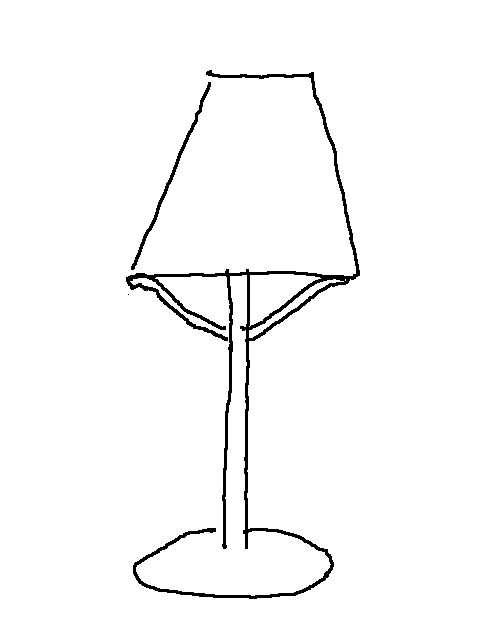
\includegraphics[width=0.95\linewidth]{image/lamps.jpg} \par
    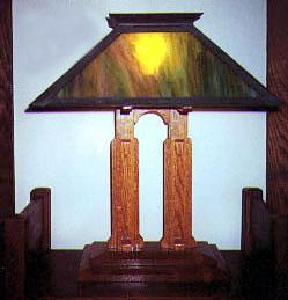
\includegraphics[width=0.95\linewidth]{image/lamp1.jpg} \par
    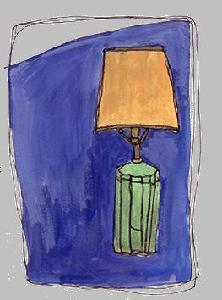
\includegraphics[width=0.95\linewidth]{image/lamp2.jpg} \par
    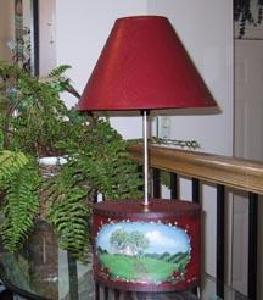
\includegraphics[width=0.95\linewidth]{image/lamp3.jpg} \par
\end{multicols}
\caption{Ejemplo de una posible búsqueda, la imagen de la izquierda representa el dibujo de búsqueda y las de la derecha los resultados esperados.}
\end{figure}

\section*{Diseño e Implementación}
	\subsection{Encontrar concordancias SIFT}

	\subsection{Cálculo de Homografía}
				
	\subsection{Unión de Imágenes}
	


\section*{Experimentación}

\section*{Conclusión}


\begin{thebibliography}{99}


\end{thebibliography}

\end{document}
